\documentclass[border=10pt]{standalone}

\usepackage{tikz}
\usepackage{tikzsymbols}
\usetikzlibrary{calc,patterns,shapes.geometric}

\def\centerarc[#1](#2)(#3:#4:#5){\draw[#1] ($(#2)+({#5*cos(#3)},{#5*sin(#3)})$) arc (#3:#4:#5);}

\begin{document}
	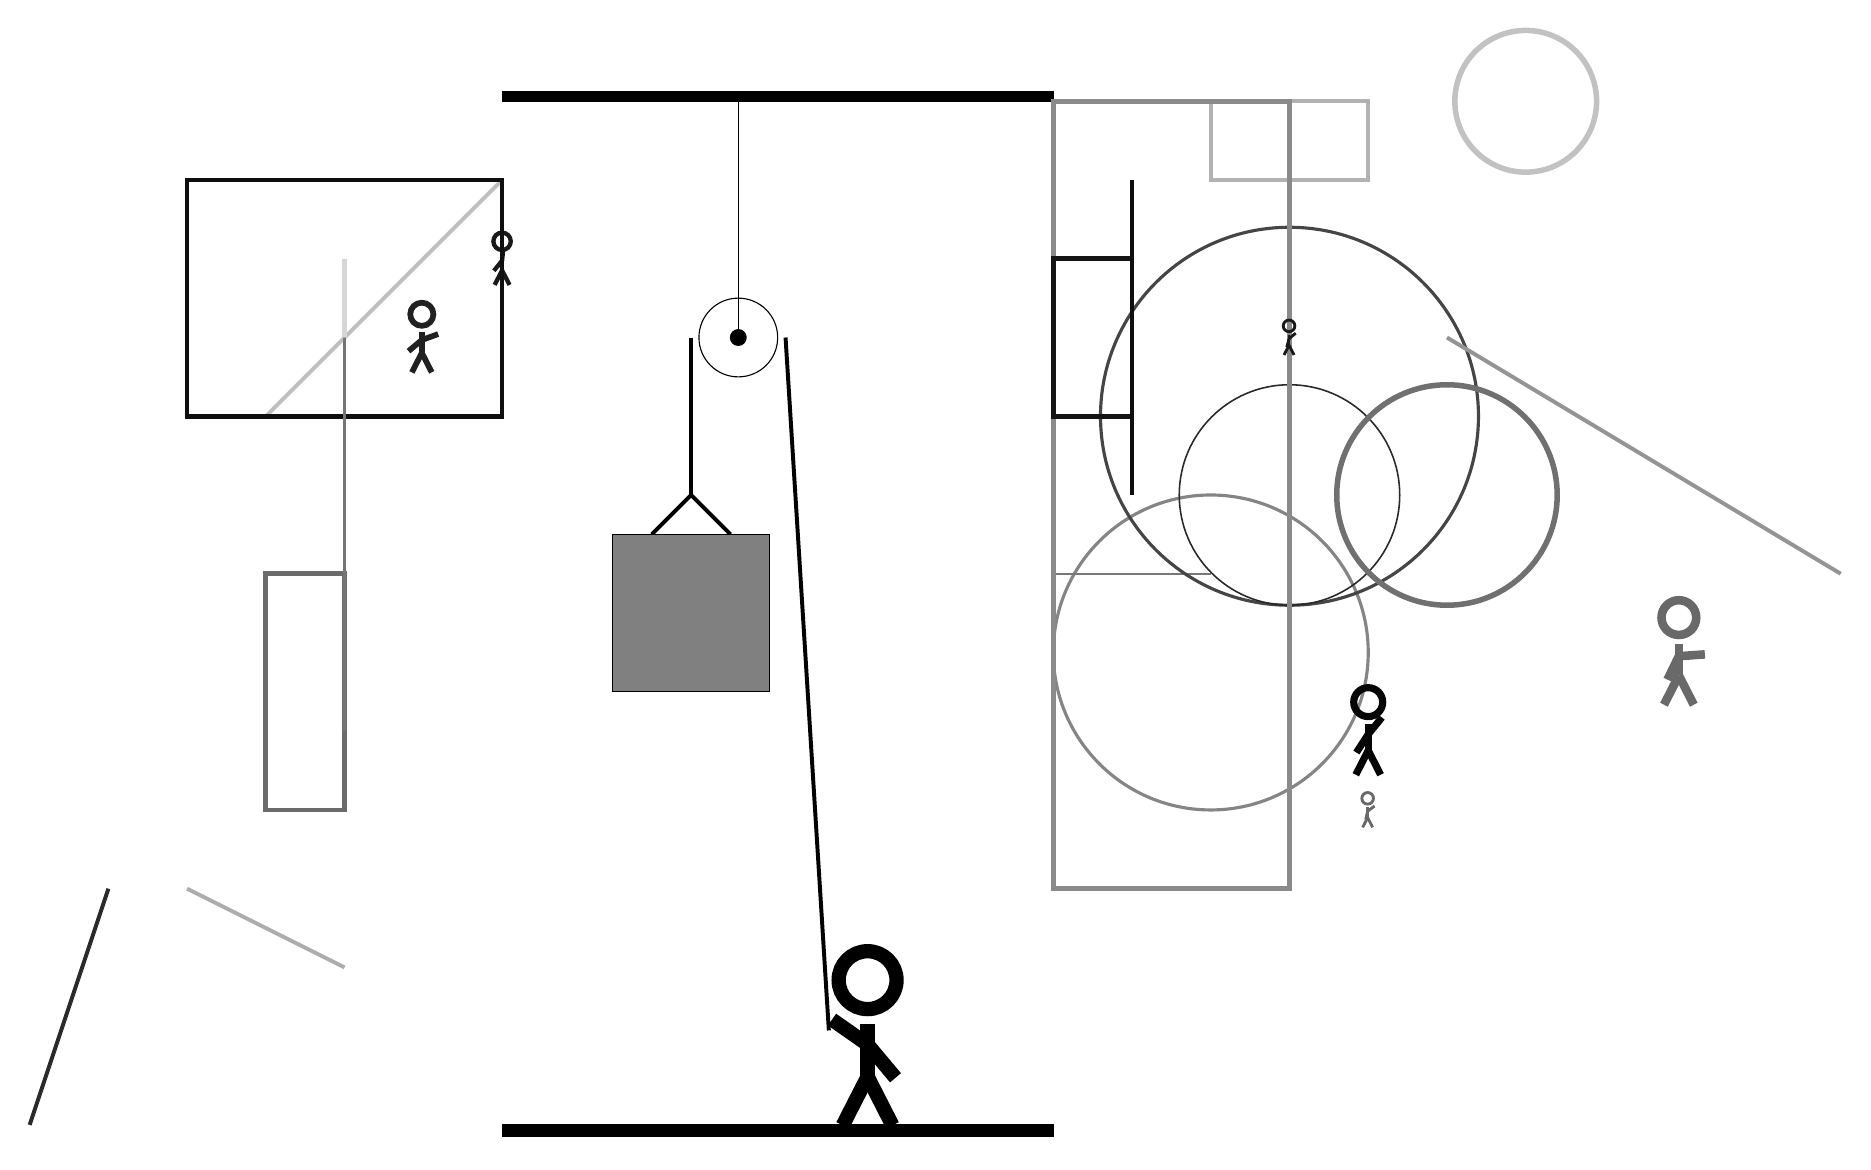
\begin{tikzpicture}
		%%%%% START %%%%%
		
		\draw[fill=black] (-2, 10) rectangle (5, 10.125);
		
		\draw (1, 7) circle (0.5);
		\draw[fill=black] (1, 7) circle (0.1);
		\draw (1, 10) -- (1, 7);
		
		\draw[line width=0.5mm] (-0.1, 4.5) -- (0.4, 5.0) -- (0.9, 4.5);
		\draw[fill=black!50] (-0.6, 4.5) rectangle (1.4, 2.5);
		
		\draw[line width=0.5mm] (0.4, 7) -- (0.4, 5.0);
		\centerarc[line width=0.5mm](1, 7)(0:180:0.6);
		\draw[line width=0.5mm](1.6, 7) -- (2.15, -1.8);
		
		\draw[line width=0.5mm, color=black!83](-7, 0) -- (-8, -3);
		
		\draw [line width=0.4mm, color=black!48](7, 3) circle (2.0);
		\node[line width=0.7mm, color=black!90] at (-2, 8) {\Strichmaxerl[3][51][84]};
		\draw [line width=0.7mm, color=black!24](11, 10) circle (0.9);
		\node[line width=0.4mm, color=black!87] at (-3, 7) {\Strichmaxerl[4][40][20]};
		\node[line width=0.6mm, color=black!59] at (13, 3) {\Strichmaxerl[6][64][4]};
		\draw[line width=0.5mm, color=black!25](-2, 9) -- (-5, 6);
		\draw[line width=0.3mm, color=black!53] (7, 4) rectangle (5, 4);
		\draw[line width=0.7mm, color=black!16] (-4, 7) rectangle (-4, 8);
		\draw[line width=0.6mm, color=black!94] (-2, 6) rectangle (-6, 9);
		\draw [line width=0.4mm, color=black!73](8, 6) circle (2.4);
		\draw[line width=0.6mm, color=black!77] (6, 4) rectangle (6, 4);
		\draw[line width=0.6mm, color=black!58] (-4, 1) rectangle (-5, 4);
		
		\node[line width=0.5mm, color=black!59] at (9, 1) {\Strichmaxerl[2][77][37]};
		\draw [line width=0.6mm, color=black!69](10, 4) circle (0.0);
		\draw [line width=0.2mm, color=black!84](8, 5) circle (1.4);
		
		\draw[line width=0.5mm, color=black!42](10, 7) -- (15, 4);
		
		\draw[line width=0.3mm, color=black!54] (-4, 7) rectangle (-4, 2);
		\node[line width=0.6mm, color=black!98] at (9, 2) {\Strichmaxerl[5][57][51]};
		\draw[line width=0.5mm, color=black!30] (7, 9) rectangle (9, 10);
		\draw[line width=0.6mm, color=black!46] (5, 10) rectangle (8, 0);
		\draw [line width=0.7mm, color=black!56](10, 5) circle (1.4);
		\draw[line width=0.6mm, color=black!92] (5, 8) rectangle (6, 6);
		\draw[line width=0.4mm, color=black!94] (6, 9) rectangle (6, 5);
		\node[line width=0.5mm, color=black!90] at (8, 7) {\Strichmaxerl[2][75][40]};
		\draw[line width=0.5mm, color=black!32](-4, -1) -- (-6, 0);
		
		
		\node at (2.6, -1.9) {\Strichmaxerl[10][-35][-50]};
		
		\draw[fill=black] (-2, -3) rectangle (5, -3.15);
		
		%%%%% END %%%%%
	\end{tikzpicture}
\end{document}